\section{Results}\label{sec:results}

\subsection{Overview of \repqa}

\repqa is a benchmark for systematically evaluating the readability of LLMs in patient education question answering.
It comprises a high-quality collection of patient education QA pairs, each with an expert-grounded reference answer, together with a large-scale set of unlabeled questions for training.
\begin{figure}[htbp]
    \centering
    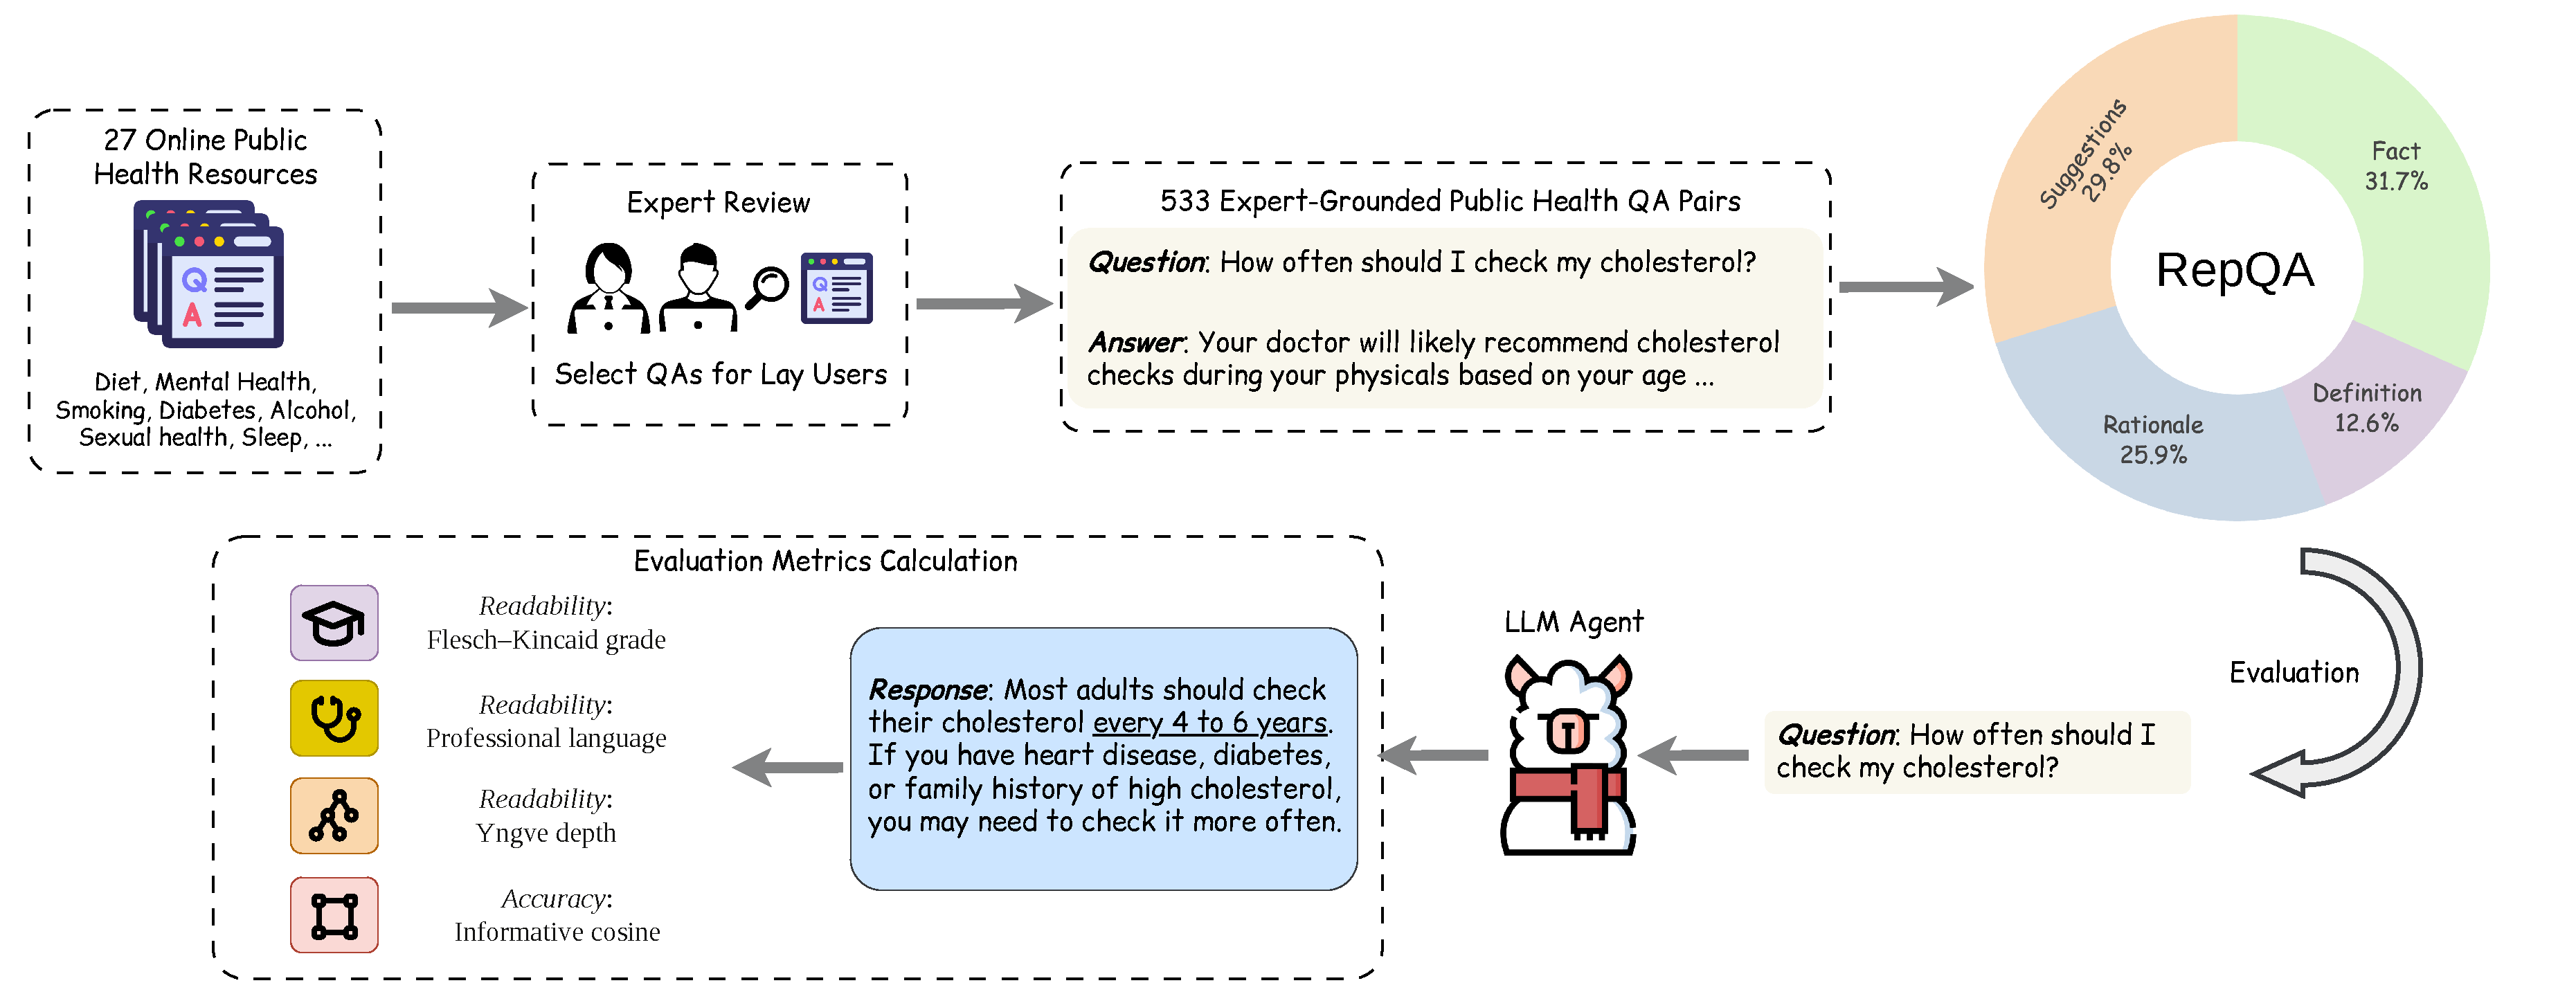
\includegraphics[width=1.0\textwidth]{figs/workflow_new.pdf}
    \caption{
        Overview of the \repqa benchmark. \textbf{Top:} dataset construction --- patient-education QA pairs are collected from 27 online public health resources and filtered by domain experts to suit lay users, yielding 533 expert-grounded QA pairs (each with an auto-generated multiple-choice counterpart) that span four categories (Suggestion, Fact, Definition, and Rationale). \textbf{Bottom:} evaluation --- given a question, an LLM agent generates a free-form response, which is scored by three readability metrics (Flesch--Kincaid grade, professional language, and Yngve depth) and an informativeness metric (the informative cosine between the response and the expert reference answer).
    }
    \label{fig:workflow}
\end{figure}

Figure~\ref{fig:workflow} illustrates the overall dataset construction and evaluation pipeline: the dataset is curated through expert review, while the evaluation involves both readability assessment and an informativeness measure against the reference answers.
The construction procedure, evaluation metrics, and study design are detailed in the Methods (Section~\ref{sec:methods}).

\begin{table*}[t]
    \centering
    \caption{Examples and distribution of question categories in \repqa. Each question is accompanied by a corresponding reference answer.}
    \resizebox{\textwidth}{!}{
    \begin{tabular}{cp{15cm}c}
    \toprule
    Category & Example \& Reference Answer & Proportion \\
    \midrule
    \midrule
    \multirow{4}{*}{Suggestion} & \textbf{Q:} How can I quit smoking? & \multirow{4}{*}{29.8\%} \\
    & \textbf{A:} Commit to a quit day, choose a method for quitting (cold turkey or weaning down), talk to your doctor about medications to help quit, make a plan for when you quit on how to resist temptations, remove triggers, and have replacement activities, and then quit on your quit day! & \\
    \midrule
    \multirow{3}{*}{Fact} & \textbf{Q:} What are the chemicals in cigarettes? &  \multirow{3}{*}{31.7\%} \\
    & \textbf{A:}There are over 7,000 chemicals in cigarettes including arsenic, formaldehyde, tar, nicotine, and carbon monoxide, all of which are dangerous to your health. & \\
    \midrule
    \multirow{4}{*}{Definition} & \textbf{Q:} What is the Mediterranean Diet? & \multirow{4}{*}{12.6\%} \\
    & \textbf{A:} A Mediterranean diet is considered a healthy option as it emphasizes fruits and vegetables, whole grains, beans and legumes, low-fat dairy products, fish and poultry, and vegetable oils. It also limits sugars, processed foods, and fatty meats. & \\
    \midrule
    \multirow{3}{*}{Rationale} & \textbf{Q:} Why is blood pressure called a "silent killer"? & \multirow{3}{*}{25.9\%} \\
    & \textbf{A:} High blood pressure is sometimes called a silent killer because it can have no physical symptoms; however, the high blood pressure can damage arteries risking serious health events like heart attack or stroke. & \\
    \bottomrule
    \end{tabular}
    }
    \label{tab:dataset_category}
\end{table*}

The evaluation set of \repqa contains 533 QA pairs curated from 27 authoritative online public health resources and reviewed by domain experts in nursing, public health, and clinical communication.
Each question is phrased in plain language, without user profiles, and is accompanied by a reference answer.
As shown in Table~\ref{tab:dataset_category}, the QA pairs span four categories that capture common types of public health inquiries from lay users: \textit{Suggestion} (questions seeking advice), \textit{Fact} (questions requesting objective, verifiable information), \textit{Definition} (questions asking for explanations of medical terms or conditions), and \textit{Rationale} (questions seeking justifications behind medical guidance).
To enable informativeness assessment of free-form responses, each QA pair includes an expert-grounded reference answer, against which a generated response is compared via the informative cosine (IC).
In addition, \repqa provides a large-scale collection of 36,060 expert-reviewed public health questions spanning topics such as sleep, exercise, smoking, weight, diet, HIV care, mental health, cardiovascular disease, diabetes, cholesterol, and SOGI, supporting the exploration of readability-enhancement strategies such as reinforcement learning with verifiable readability rewards.

Using \repqa, we studied three research questions concerning LLMs' ability to adapt, assess, and optimize readability:
(RQ1) can LLMs generate responses at a specified reading level?
(RQ2) can LLMs determine what readability is needed for a given question?
and (RQ3) can readability serve as a reward signal?
We evaluated 19 LLMs, including 5 proprietary models and 14 open-source models, alongside five readability-enhancement strategies. The full experimental setup, including the list of evaluated models and configurations, is provided in Section~\ref{sec:exp_setup}.

\subsection{LLMs struggle to generate responses at a specified reading level}

People with different educational backgrounds have varying health literacy, so a healthcare agent should be able to adapt the readability of its answers to a requested level (RQ1).
We set a target score, i.e., 6 for the Flesch–Kincaid (FK) grade level and 0 for the professional-language (PL) score, and prompted each model to answer the queries accordingly. $\pi{=}6$ approximates a 5th-grade level intended to be broadly accessible, and $\rho{=}0$ denotes the absence of medical jargon.
As shown in Table~\ref{tab:repqa-main}, most models struggled to hit the target, often overshooting complexity or, when simplifying, omitting qualifiers.
Across the four categories, \textit{definition} was the easiest, with the lowest readability scores.

\begin{table*}[t]
\centering
\caption{Benchmarking proprietary and open-source LLMs with the \repqa{} metric suite. PL = Professional Language ($\downarrow$ less jargon), FK = Flesch--Kincaid Grade (target $\approx 6$), YD = Yngve Depth ($\downarrow$ simpler syntax), IC = Informative Cosine ($\uparrow$ more informative).}
\label{tab:repqa-main}
\small
\setlength{\tabcolsep}{3pt}
\resizebox{\linewidth}{!}{
\begin{tabular}{l cccc cccc cccc cccc}
\toprule
 & \multicolumn{4}{c}{Suggestion} & \multicolumn{4}{c}{Fact} & \multicolumn{4}{c}{Rationale} & \multicolumn{4}{c}{Definition} \\
\cmidrule(lr){2-5} \cmidrule(lr){6-9} \cmidrule(lr){10-13} \cmidrule(lr){14-17}
Model & PL$\downarrow$ & \textbf{FK$\rightarrow6$} & YD$\downarrow$ & IC$\uparrow$ & PL$\downarrow$ & \textbf{FK$\rightarrow6$} & YD$\downarrow$ & IC$\uparrow$ & PL$\downarrow$ & \textbf{FK$\rightarrow6$} & YD$\downarrow$ & IC$\uparrow$ & PL$\downarrow$ & \textbf{FK$\rightarrow6$} & YD$\downarrow$ & IC$\uparrow$ \\
\midrule
\multicolumn{17}{c}{\textbf{Proprietary Models (latest)}} \\
\midrule
GPT-5.5 & 2.55 & 11.08 & \underline{0.19} & 0.67 & 3.44 & 14.19 & \underline{1.11} & 0.74 & \underline{5.51} & 12.00 & 0.29 & \underline{0.75} & \underline{5.40} & 11.78 & \textbf{0.07} & 0.77 \\
GPT-5.4 & 2.08 & 15.90 & 1.67 & 0.67 & \textbf{2.65} & 15.00 & 1.29 & 0.74 & \textbf{4.33} & 13.68 & \underline{0.26} & 0.74 & \textbf{5.24} & 13.53 & 0.76 & 0.77 \\
GPT-5.1 & 2.24 & \textbf{8.24} & \textbf{0.04} & 0.65 & \underline{3.02} & \textbf{11.11} & \textbf{0.54} & 0.74 & 5.85 & \textbf{9.01} & \textbf{0.00} & 0.74 & 6.05 & \underline{10.90} & \underline{0.19} & 0.78 \\
GPT-4.1 & \textbf{1.62} & \underline{8.30} & 1.36 & \underline{0.71} & 3.12 & \underline{11.37} & 3.22 & \textbf{0.78} & 6.36 & \underline{9.84} & 2.42 & \textbf{0.77} & 7.50 & 10.95 & 2.58 & \underline{0.81} \\
GPT-4.1-mini & \underline{2.02} & 9.15 & 1.93 & \textbf{0.72} & 4.14 & 11.49 & 3.22 & \underline{0.77} & 7.01 & 10.70 & 3.06 & \textbf{0.77} & 8.56 & \textbf{10.71} & 2.92 & \textbf{0.82} \\
\midrule
\multicolumn{17}{c}{\textbf{Open-Source Models}} \\
\midrule
LLaMA3.1-8B & 2.08 & 8.15 & 0.28 & 0.68 & 3.89 & 9.21 & 0.62 & 0.75 & 7.12 & 9.39 & 0.50 & 0.74 & 7.87 & 10.44 & 1.01 & 0.79 \\
Qwen2.5-7B & 1.75 & \textbf{7.72} & 1.21 & 0.69 & 3.64 & 9.99 & 2.83 & \textbf{0.77} & 6.33 & 9.79 & 2.70 & \textbf{0.76} & 7.54 & 10.26 & 3.04 & \underline{0.81} \\
BioMistral-7B & 2.88 & 8.70 & 3.05 & 0.67 & 4.08 & 9.50 & 3.50 & 0.73 & 7.97 & \underline{9.37} & 2.98 & 0.72 & 8.05 & 10.38 & 3.08 & 0.78 \\
Phi-4 & 1.56 & 8.03 & 0.28 & 0.69 & 3.58 & 9.54 & 1.05 & \underline{0.76} & 6.72 & 10.07 & 0.95 & \underline{0.75} & 7.09 & 11.00 & 1.78 & 0.80 \\
Yi-1.5-9B & 1.83 & 9.17 & 1.52 & 0.69 & 4.52 & 10.21 & 2.64 & \underline{0.76} & 6.72 & 10.57 & 2.52 & 0.74 & 8.52 & 11.50 & 2.75 & 0.80 \\
Mistral-7B & 1.97 & 8.10 & 1.22 & 0.68 & 3.76 & 9.27 & 2.25 & \underline{0.76} & 7.10 & 10.52 & 2.58 & \underline{0.75} & 8.18 & 10.81 & 2.82 & 0.80 \\
InternLM3-8B & \underline{1.53} & 8.38 & \textbf{0.04} & 0.67 & 2.98 & 9.52 & \underline{0.22} & 0.73 & 5.38 & 10.13 & \underline{0.10} & 0.73 & \textbf{4.65} & 11.04 & \underline{0.77} & 0.77 \\
Gemma-3-12B & 1.59 & 7.97 & 0.29 & 0.66 & \underline{2.09} & \textbf{8.60} & 1.14 & 0.74 & \underline{5.33} & \textbf{8.78} & 1.02 & 0.73 & \underline{4.92} & \textbf{8.77} & 1.10 & 0.79 \\
Qwen2.5-14B & 2.03 & 8.33 & 1.36 & \underline{0.70} & 3.42 & 9.61 & 2.38 & \textbf{0.77} & 6.26 & 10.20 & 2.68 & \textbf{0.76} & 6.89 & 11.05 & 3.21 & \underline{0.81} \\
Qwen2.5-32B & \textbf{1.34} & \underline{7.90} & 1.18 & \textbf{0.71} & 3.45 & 9.66 & 2.47 & \textbf{0.77} & 5.80 & 10.39 & 2.77 & \textbf{0.76} & 6.71 & 10.48 & 2.94 & \underline{0.81} \\
% \multicolumn{17}{c}{\textbf{Newly Added Open-Source Models}} \\
% \midrule
Qwen3-8B & 2.11 & 8.45 & 1.65 & \underline{0.70} & 3.39 & 10.76 & 3.06 & \textbf{0.77} & 7.55 & 10.32 & 2.41 & \textbf{0.76} & 7.16 & 10.73 & 2.61 & \textbf{0.82} \\
Qwen3-14B & 1.78 & 7.93 & 1.04 & \underline{0.70} & 3.30 & 10.79 & 2.39 & \textbf{0.77} & 6.47 & 10.64 & 2.16 & \textbf{0.76} & 8.66 & 10.69 & 2.13 & \underline{0.81} \\
Qwen3-32B & 2.08 & 8.08 & 0.76 & \underline{0.70} & 3.31 & 10.32 & 1.69 & \textbf{0.77} & 6.18 & 10.55 & 1.51 & \textbf{0.76} & 8.17 & 11.06 & 2.00 & 0.80 \\
Gemma-3-27B & 1.58 & 8.28 & \underline{0.11} & 0.66 & \textbf{1.77} & \underline{9.12} & \textbf{0.14} & 0.74 & \textbf{4.15} & 9.38 & \textbf{0.00} & 0.71 & 5.04 & \underline{9.12} & \textbf{0.00} & 0.78 \\
\bottomrule
\end{tabular}
}
\end{table*}

To further probe readability control, we evaluated a set of representative models, spanning non-thinking models (LLaMA~3.1-8B, Qwen-3-30B) and thinking models (DeepSeek-R1-Distill-Qwen, Qwen-3-30B-Thinking, GPT-4.1), focusing on their ability to match requested reading levels.
We set four target levels, i.e., 5th grade, middle school, high school, and college, corresponding to FK grade levels of 6, 9, 12, and 15.
\begin{figure}[htbp]
    \centering
    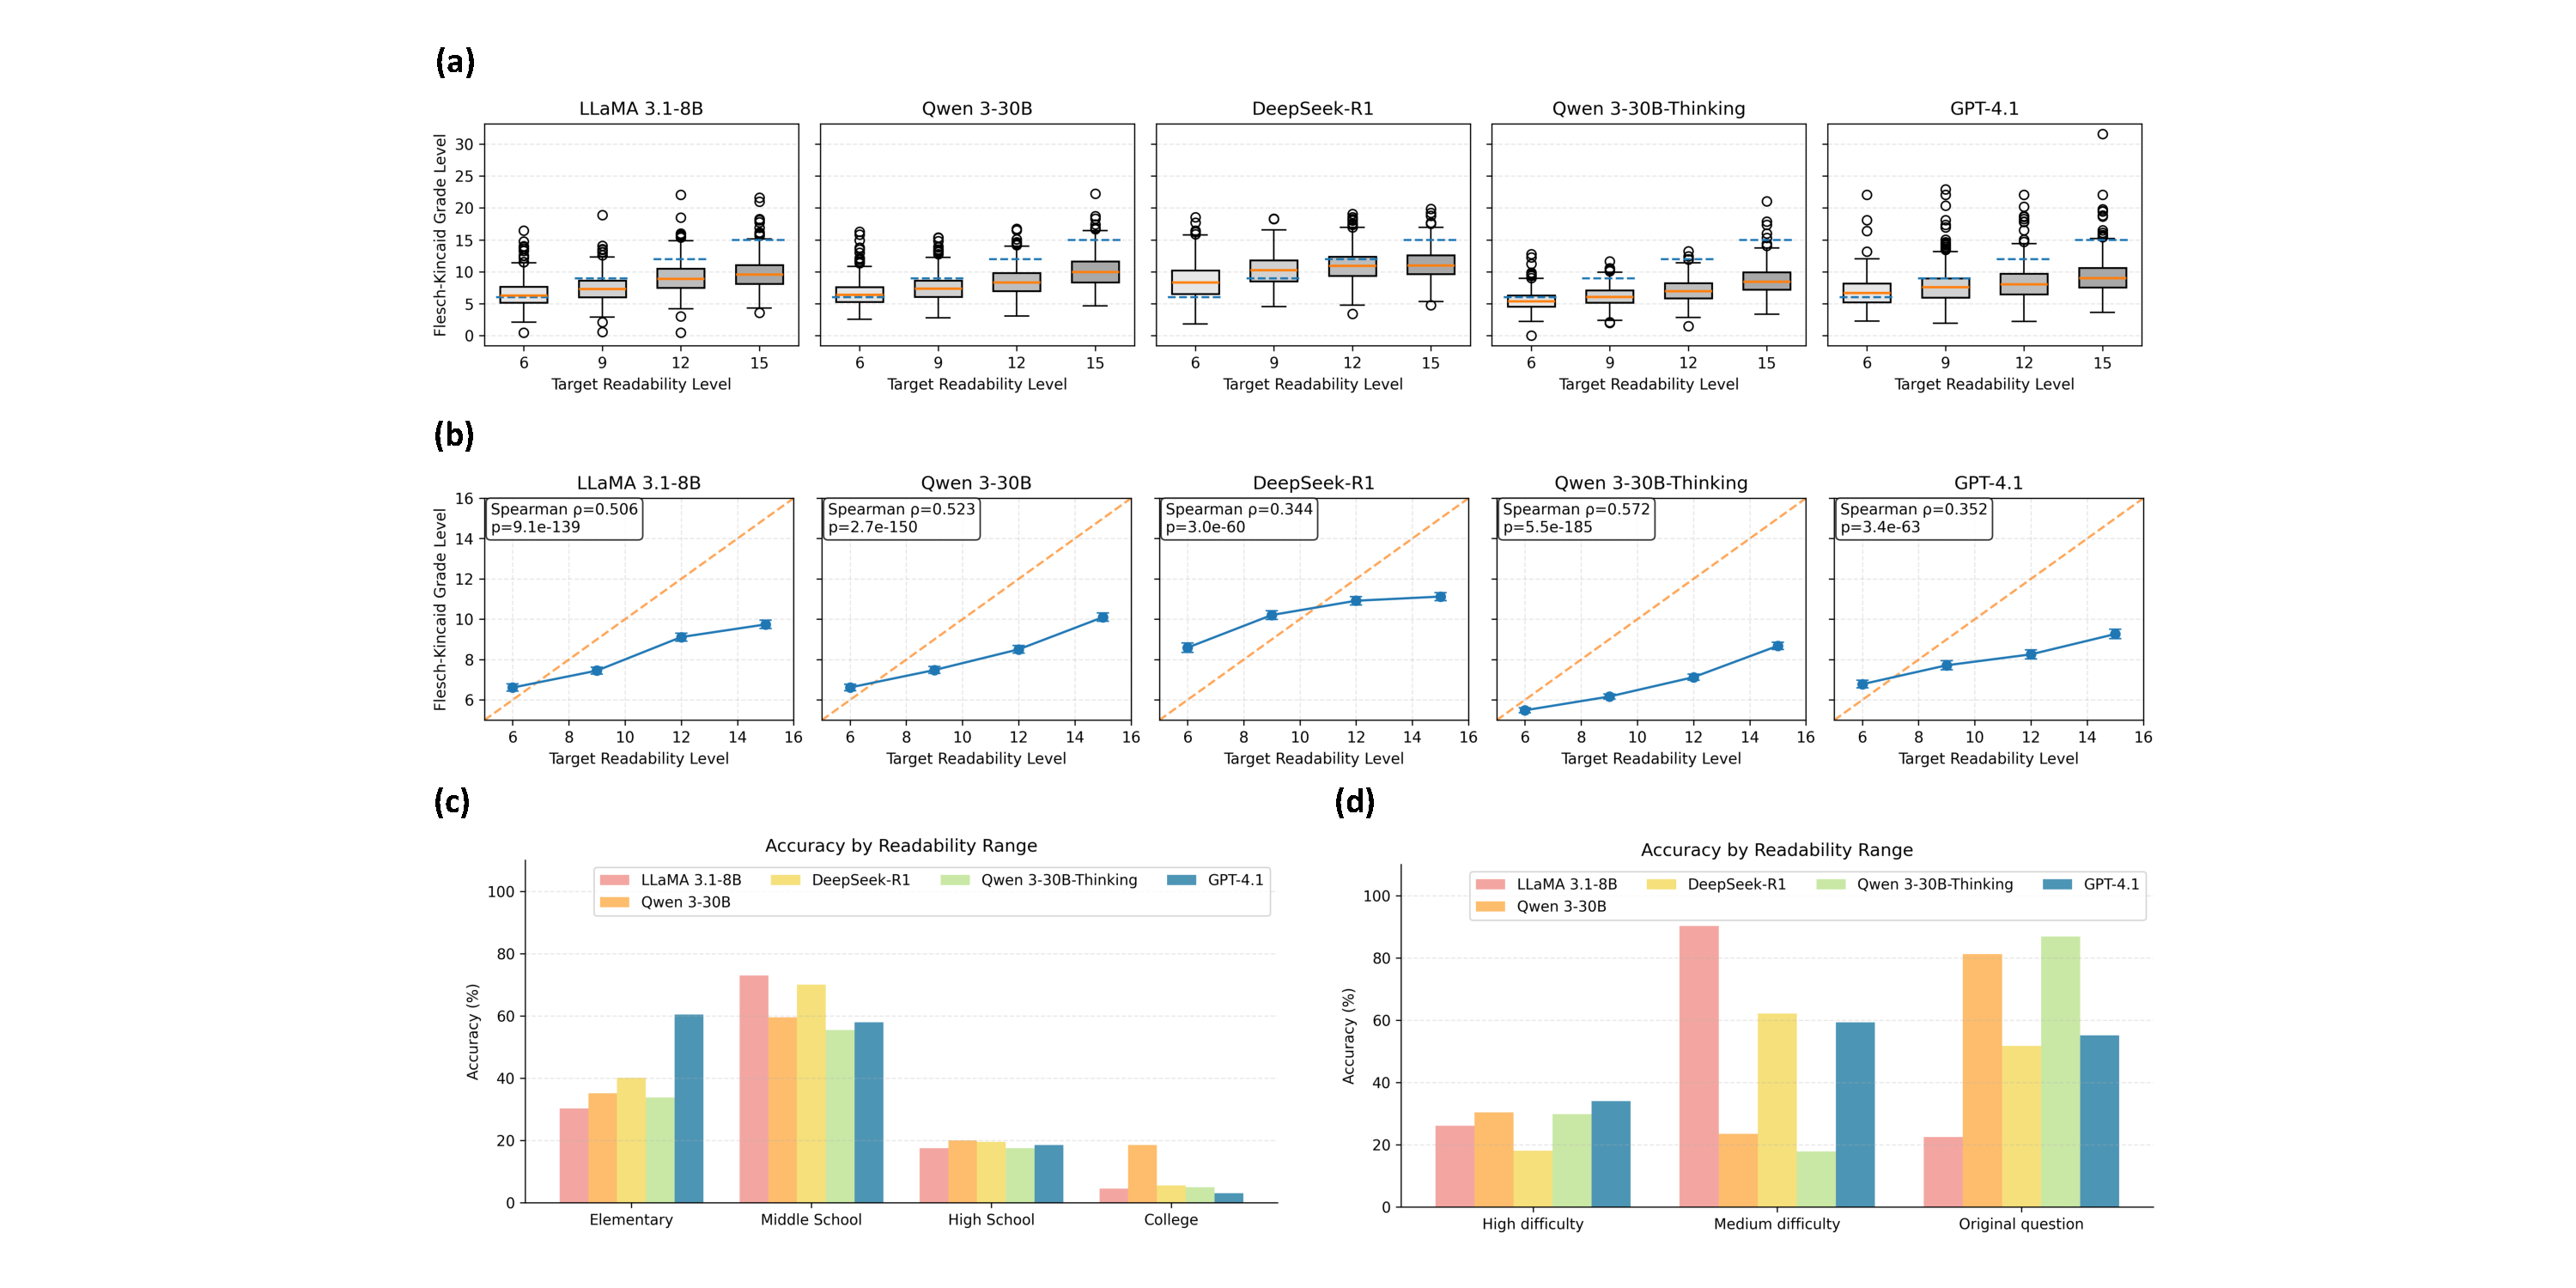
\includegraphics[width=1.0\linewidth]{figs/readability_study_new.pdf}
    \caption{
    Readability control and understanding across five models.
    \textbf{(a)} Achieved Flesch–Kincaid grades when instructed to write at target levels 6/9/12/15 (boxplots). Red horizontal lines mark the targets, and blue dashed lines mark the per-target mean grade.
    \textbf{(b)} Mean Flesch–Kincaid grade vs.\ target (error bars show 95\% CI).
    \textbf{(c)} Accuracy of classifying generated responses into Flesch–Kincaid buckets (Elementary/Middle/High/College).
    \textbf{(d)} Accuracy when classifying Original/Medium/High counterparts of the same question.
    }
    \label{fig:analysis}
\end{figure}

As shown in Figure~\ref{fig:analysis}(a,b), all models generally followed the intended direction (Spearman $\rho\approx 0.34\sim0.57$) but remained poorly calibrated: their FK grades consistently fell short of the targets, with larger deviations at higher levels.
In short, while models adjusted readability \emph{relatively}, they failed in \emph{absolute} alignment.

\subsection{LLMs poorly identify the readability required for a question}

We next examined whether poor control stems from a weak understanding of readability (RQ2).
We first tested whether models can recognize the reading level of existing text: we sampled 200 generated responses per bin (Elementary, Middle School, High School, College; mapped from FK grade) and asked models to classify the bin.
As shown in Figure~\ref{fig:analysis}(c), accuracy peaked at Middle School, was moderate at Elementary, and collapsed at High School and College.
This systematic bias toward lower buckets mirrored the undershoot observed for readability control.

We then studied whether LLMs understand differences in the medical knowledge required by a question.
For each question in \repqa, we prompted GPT-4o to generate two counterparts that vary only in the required domain knowledge (Medium and High).
Each model then classified the resulting variant.
As shown in Figure~\ref{fig:analysis}(d), performance was uneven across systems, e.g., LLaMA~3.1-8B was relatively strong on Medium but weak on Original, whereas Qwen-3-30B-Thinking excelled on Original yet remained low on High.
Across models, detection of High difficulty was uniformly poor, indicating limited sensitivity to advanced domain knowledge and helping explain the tendency to default to overly simple outputs.

\subsection{Readability can serve as a reward signal, but at an accuracy cost}

Reinforcement learning has shown promise for steering LLMs toward preferred behaviors. We therefore studied whether readability can act as a useful reward signal (RQ3).
We optimized readability using the reward in Eq.~\ref{equ:reward} within two reinforcement-learning algorithms, GRPO~\citep{shao2024deepseekmath} and DAPO~\citep{yu2025dapo}, the latter improving upon GRPO with decoupled clipping and dynamic sampling (Methods, Section~\ref{sec:methods}).
As training-free baselines we included three readability-control methods from \citet{ribeiro-etal-2023-generating}: \emph{Prompt} (instruction-based control, prompting the base model for simple, plain-language answers), \emph{CoT} (chain-of-thought prompting), and \emph{Lookahead} (a decoding method that at each step estimates the readability of candidate continuations via a short greedy lookahead and biases generation toward the target grade level). All three were applied to the base model with no fine-tuning.
Results are reported in Table~\ref{tab:post}.

The training-free controls traded off differently across the readability axes.
\emph{Prompt} sharply lowered the word-level grade (FK) and jargon (PL), but raised syntactic complexity (YD) and eroded informativeness (IC); \emph{Lookahead} pulled FK toward the target while best preserving IC among the non-RL methods, yet left jargon and syntax largely unchanged because its guidance optimizes FK alone; and \emph{CoT} produced less readable text with no meaningful gain in informativeness.
In contrast, RL fine-tuning (GRPO/DAPO) was the only approach that improved all four axes at once -- lowering FK, PL, and YD while retaining the highest IC -- since its reward jointly targets word choice, syntax, and faithfulness.
Both GRPO and DAPO improved readability; among them, DAPO yielded the largest gains, reducing the grade level by 41.4\% on average and the professional-language score by 73.3\%.
Moreover, DAPO outperformed vanilla GRPO on professional-language readability (53.4\% average reduction) while maintaining a comparable grade level (3.0\% difference).
Although RL fine-tuning largely retained informativeness (IC) at the aggregate level, the drive toward simpler text can still cost content fidelity: as the case study (Section~\ref{sec:case_study}) and the expert evaluation below show, the simplified responses sometimes omitted key facts, especially on \textit{Suggestion} and \textit{Fact}, highlighting the difficulty of simplifying without losing content.

\begin{table*}[t]
\centering
\caption{Readability-control strategies on the \repqa{} metric suite, per question type. For each base model we compared training-free controls -- \emph{Prompt} (instruction-based control), \emph{CoT} (chain-of-thought), and \emph{Lookahead} (readability-guided lookahead decoding, \citealp{ribeiro-etal-2023-generating}) -- against RL fine-tuning (\emph{DAPO}/\emph{GRPO}). PL = Professional Language ($\downarrow$), FK = Flesch--Kincaid Grade (target $\approx 6$), YD = Yngve Depth ($\downarrow$, raw), IC = Informative Cosine ($\uparrow$). Prompting and lookahead improve word-level readability (FK) but not syntactic complexity (YD); RL improves all axes while best retaining informativeness (IC). Within each base model, \textbf{bold} marks the best and \underline{underline} the second-best value per column.}
\label{tab:post}
\tiny
\setlength{\tabcolsep}{3pt}
\begin{tabular}{l cccc cccc cccc cccc}
\toprule
 & \multicolumn{4}{c}{Suggestion} & \multicolumn{4}{c}{Fact} & \multicolumn{4}{c}{Rationale} & \multicolumn{4}{c}{Definition} \\
\cmidrule(lr){2-5} \cmidrule(lr){6-9} \cmidrule(lr){10-13} \cmidrule(lr){14-17}
Model & PL$\downarrow$ & FK$\rightarrow6$ & YD$\downarrow$ & IC$\uparrow$ & PL$\downarrow$ & FK$\rightarrow6$ & YD$\downarrow$ & IC$\uparrow$ & PL$\downarrow$ & FK$\rightarrow6$ & YD$\downarrow$ & IC$\uparrow$ & PL$\downarrow$ & FK$\rightarrow6$ & YD$\downarrow$ & IC$\uparrow$ \\
\midrule
LLaMA3.1-8B & 2.08 & 8.15 & 0.28 & 0.68 & 3.89 & 9.21 & 0.62 & 0.75 & 7.12 & 9.39 & 0.50 & 0.74 & 7.87 & 10.44 & 1.01 & 0.79 \\
\scriptsize + Prompt & \underline{0.90} & 5.24 & 0.50 & 0.66 & 1.69 & 7.12 & 1.83 & 0.73 & 3.98 & 5.75 & 1.58 & 0.73 & 5.76 & \textbf{5.99} & 1.65 & 0.79 \\
\scriptsize + CoT & 3.08 & 10.25 & 4.11 & 0.61 & 2.22 & 9.89 & 3.90 & 0.70 & 5.22 & 9.65 & 3.28 & 0.70 & 8.85 & 9.65 & 3.07 & 0.76 \\
\scriptsize + Lookahead & 2.24 & 6.48 & 0.28 & 0.68 & 4.05 & 6.65 & 0.77 & 0.75 & 6.55 & 6.86 & 0.28 & 0.74 & 8.28 & 6.93 & 1.21 & 0.77 \\
\scriptsize + DAPO & \textbf{0.76} & \underline{5.83} & \textbf{0.02} & \textbf{0.72} & \textbf{0.57} & \underline{5.92} & \textbf{0.08} & \textbf{0.78} & \textbf{1.54} & \textbf{5.91} & \textbf{0.02} & \textbf{0.76} & \textbf{2.52} & \underline{6.20} & \textbf{0.12} & \underline{0.80} \\
\scriptsize + GRPO & 1.07 & \textbf{5.92} & \underline{0.13} & \underline{0.70} & \underline{1.64} & \textbf{5.92} & \underline{0.35} & \underline{0.76} & \underline{3.07} & \underline{5.88} & \underline{0.08} & \underline{0.75} & \underline{5.41} & 6.83 & \underline{0.46} & \textbf{0.81} \\
\midrule
Qwen3-8B & 2.11 & 8.45 & \underline{1.65} & \underline{0.70} & 3.39 & 10.76 & 3.06 & \underline{0.77} & 7.55 & 10.32 & \underline{2.41} & \underline{0.76} & 7.16 & 10.73 & 2.61 & \textbf{0.82} \\
\scriptsize + Prompt & \textbf{0.69} & 4.61 & 2.57 & 0.66 & \underline{1.33} & 5.10 & \underline{2.58} & 0.73 & \underline{3.17} & 5.33 & 2.52 & 0.72 & \textbf{3.86} & \textbf{5.14} & \underline{2.40} & 0.77 \\
\scriptsize + CoT & 1.67 & \underline{6.62} & 3.47 & 0.59 & 2.75 & \underline{6.82} & 3.07 & 0.74 & 6.39 & \textbf{6.44} & 2.62 & 0.71 & 5.26 & \underline{7.34} & 2.63 & 0.76 \\
\scriptsize + Lookahead & 2.00 & 6.73 & \textbf{1.04} & 0.70 & 3.54 & 7.57 & \textbf{2.09} & 0.76 & 5.90 & 7.92 & \textbf{2.29} & 0.75 & 6.55 & 8.25 & \textbf{2.38} & 0.80 \\
\scriptsize + DAPO & \underline{0.79} & \textbf{6.19} & 2.82 & 0.69 & \textbf{0.71} & \textbf{6.29} & 2.82 & 0.76 & \textbf{3.03} & \underline{6.45} & 2.67 & 0.73 & \underline{4.24} & 7.37 & 2.85 & 0.80 \\
\scriptsize + GRPO & 2.11 & 8.94 & 3.19 & \textbf{0.71} & 2.41 & 9.12 & 3.23 & \textbf{0.78} & 5.17 & 9.29 & 2.94 & \textbf{0.76} & 6.16 & 9.68 & 2.99 & \underline{0.81} \\
\midrule
Qwen3-4B & 1.80 & 7.97 & \underline{1.77} & 0.69 & 3.38 & 9.76 & 3.28 & \underline{0.77} & 7.90 & 9.75 & 2.55 & \textbf{0.76} & 6.56 & 9.87 & 2.65 & \underline{0.81} \\
\scriptsize + Prompt & 0.98 & 3.34 & 2.26 & 0.63 & \underline{1.32} & 4.62 & \underline{2.51} & 0.73 & \underline{3.55} & 4.39 & 2.40 & 0.71 & \underline{4.33} & \underline{4.39} & \textbf{2.36} & 0.76 \\
\scriptsize + CoT & \textbf{0.60} & \textbf{6.44} & 3.72 & 0.57 & 1.84 & \textbf{6.83} & 3.19 & 0.72 & 5.97 & \textbf{6.48} & 2.76 & 0.70 & 5.95 & \textbf{7.35} & 2.73 & 0.76 \\
\scriptsize + Lookahead & 1.93 & \underline{6.77} & \textbf{1.34} & \underline{0.70} & 3.32 & 7.58 & 2.83 & 0.76 & 5.78 & 7.81 & \textbf{2.19} & 0.75 & 6.13 & 7.82 & 2.61 & 0.79 \\
\scriptsize + DAPO & \underline{0.68} & 7.00 & 2.48 & 0.68 & \textbf{0.75} & \underline{7.14} & \textbf{2.47} & 0.76 & \textbf{2.19} & \underline{7.17} & \underline{2.36} & 0.73 & \textbf{3.43} & 7.75 & \underline{2.43} & 0.80 \\
\scriptsize + GRPO & 1.84 & 9.25 & 3.33 & \textbf{0.71} & 1.38 & 9.22 & 3.31 & \textbf{0.77} & 4.59 & 9.08 & 2.99 & \underline{0.75} & 5.74 & 9.72 & 2.96 & \textbf{0.81} \\
\bottomrule
\end{tabular}
\end{table*}

\paragraph{Expert evaluation}
We performed a manual inspection of the responses from Qwen2.5-7B and LLaMA3.1-8B, both post-trained via DAPO.
Specifically, we presented questions to 8 domain experts in a blind evaluation, in which experts were asked to select the superior response from a pair of randomized outputs.
Our results showed that in 75\% of the cases, experts favored the responses from LLaMA3.1-8B over those from Qwen2.5-7B.
This discrepancy with the metric-based ranking in Table~\ref{tab:post} suggested that static readability metrics may deviate from human perception.

\subsection{Case study: improved readability at the expense of informativeness}\label{sec:case_study}

\repqa revealed that, although GRPO/DAPO with a readability-based reward markedly improved readability, it can reduce the informativeness of responses.
\begin{figure}[htbp]
    \centering
    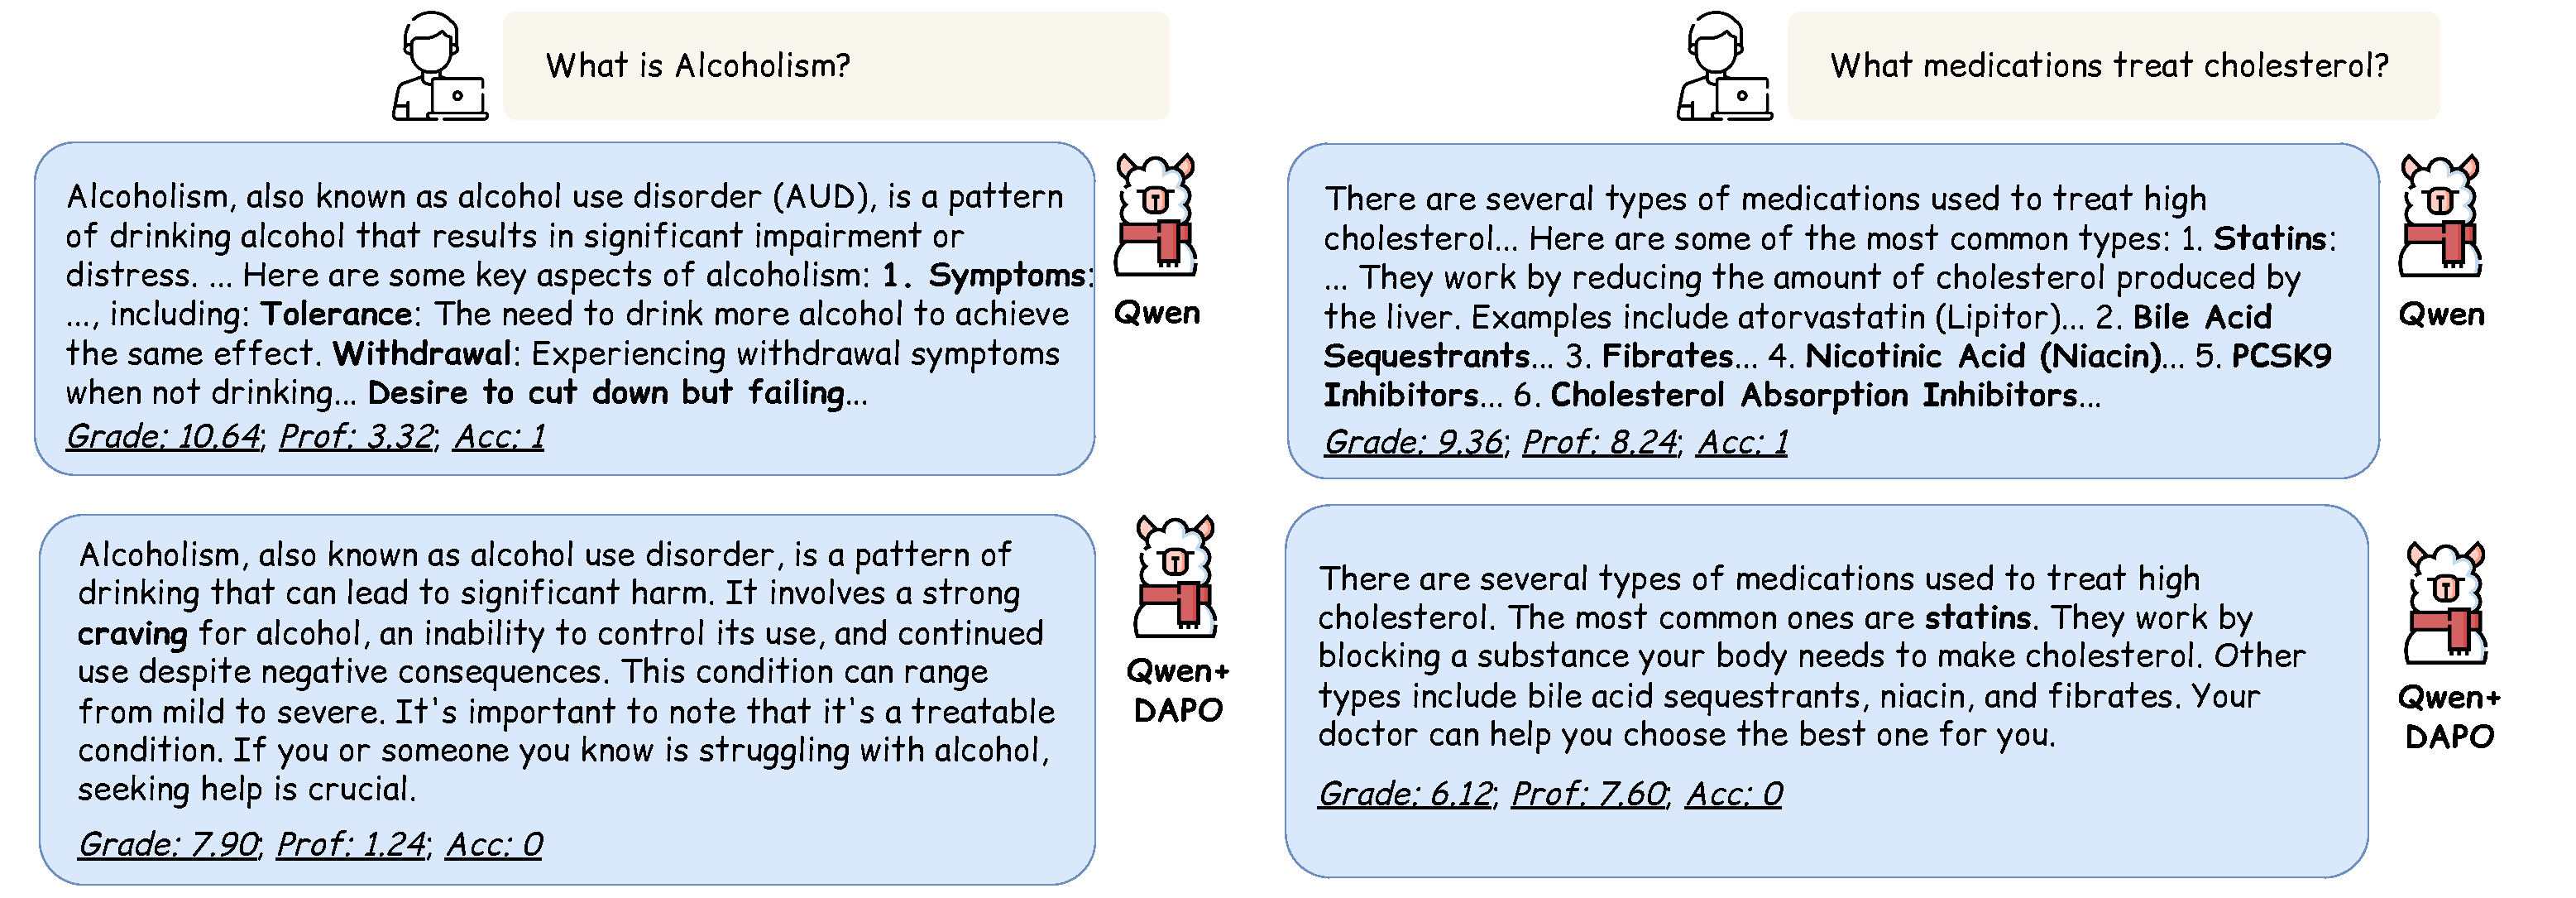
\includegraphics[width=1.\linewidth]{figs/fail_case_studyv2.pdf}
    \caption{Examples of improved readability but reduced accuracy.}
    \label{fig:fail_case}
\end{figure}

To illustrate this trade-off, Figure~\ref{fig:fail_case} presented two cases where DAPO yielded simpler text but missed key facts relative to the base model.
In particular, the DAPO model tended to over-simplify, compressing lists and collapsing categories, so that only a salient term was retained (e.g., \emph{craving} for alcohol use disorder; \emph{statins} for cholesterol drugs) while other classes (e.g., bile-acid sequestrants, fibrates, niacin, PCSK9 inhibitors) were merged into a single undifferentiated sentence, leading to information loss.
